\chapter{2006 North American Monsoon Case Study} \label{ch:2006}

\ifpdf
    \graphicspath{{Chapter_2006/figures/PNG/}{Chapter_2006/figures/PDF/}{Chapter_2006/figures/}}
\else
    \graphicspath{{Chapter_2006/figures/EPS/}{Chapter_2006/figures/}}
\fi

The recurring upper tropospheric ozone enhancements during North American Monsoon (NAM) seasons have been extensively studied by \citet{Li:2005ss}, \citet{Cooper:2006dq,Cooper:2007cr,Cooper:2009nx}, and \citet{Barth:2012qf}. Other studies have also highlighted the relevance of this feature \citep[e.g.][]{Hudman:2007fu,Choi:2009bh,Jourdain:2010tw}. While previous studies produced results that have been used to infer the climatological impact of the upper tropospheric ozone enhancement on the radiative balance, a closer look at model outputs reveals substantial variabilities. To further the understanding of a chemistry model's capability in capturing the necessary details, this study intends to perform simulations using WRF-Chem \citep{Grell:2005fv} over July and August of 2006. The period covered by this study is chosen to capture substantial anticyclonic recirculation in the upper-air, which has been shown to enhance ozone production \citep{Cooper:2007cr}.

The case study simulation results are compared against several independent data sets to identify any biases or deficiencies in the
model that have implications on the modeled ozone budget. In addition, sensitivity simulations are also performed to evaluate the relative
sensitivity of the simulated ozone distributions to emission scenarios of anthropogenic, biogenic, and lightning sources. The results from
these simulations are used to bound the range of uncertainty as well as to address the impact from potential changes in emission scenarios
in the future.

The first section of this chapter describes the model settings used in this study (\sect{2006/method}). Then, a general description of the model outputs and corresponding validation against various empirical data sets is given in Section \ref{sec:2006/general}. Once the model's performance has been evaluated, Section \ref{sec:2006/discussion} describes the core results derived from the base case simulation. Finally, this chapter is concluded with sets of sensitivity tests for determining ozone's variability with respect to  lightning-generated \chem{NO_x} (\lnox) emissions (\ssect{2006/sens/lnox}), anthropogenic emissions (\ssect{2006/sens/anthrop}), and biogenic emissions (\ssect{2006/sens/bio}).

\section{Model description}\label{sec:2006/method}

\figuremacroN{domain}{2006 case study model domain}{\label{fig:2006/domain}WRF-Chem model domain (red). Marked inner region (blue) is the primary area used for various analysis in Section \ref{sec:2006/discussion}.\vspace{-.2in}}

Simulations are performed with the Weather Research and Forecasting model \citep{Skamarock:2008xx} with Chemistry
\citep[WRF-Chem;][]{Grell:2005fv} version 3.4.1 over July and August, 2006. The model is configured with a horizontal grid
spacing of 36\,\unit{km} on a Lambert conformal projection centered over the contiguous United States (CONUS) as shown
in Figure \ref{fig:2006/domain}. Vertical levels are discretized on a eta coordinate with a terrain-following surface and a fixed
top at 10\,\unit{hPa}.

Meteorology is initialized and assimilated with data from National Center for Environmental Prediction (NCEP) Global Forecasting
System (GFS) final (FNL) gridded analysis at 6-hr intervals (00, 06, 12, 18\,\unit{UTC}). Nudging is performed for temperature and
water vapor above the planetary boundary layer (PBL). Nudging for horizontal winds is performed above model level 10.\footnote{At
this model level, mean and standard deviation of pressure and height are $843\pm55\,\unit{hPa}$ and $1.6\pm0.6\,\unit{km}$.}
Advection of moisture, scalar, chemical, and tracer variables are performed with positive-definite and monotonic limiters described in
\citet{Skamarock:2006wm}.

Descriptions of some of the pertinent model settings and options are given in the following section. The full namelist
template for the base case simulation is provided in Appendix \ref{apdx:namelist}.

\subsection{Model options and parameterizations}\label{ssec:2006/method/settings}

	For convective parameterization, we use the Grell-3 (G-3) scheme, a modified version of the \citet{Grell:2002bs} ensemble scheme. It uses a 144 ($=3\times3\times16$) dynamic control and static control/feedback closures with varying parameters. In addition, shallow convection is also enabled to permit less severe convective activities. For cloud microphysics, the \citet{Thompson:2008vn} scheme is used, which allows a generalized gamma distribution for graupel.

	Shortwave radiative transfer uses the Goddard two-stream method described by \citet{Chou:1998kx} with 11 bands using
	a $\delta$-Eddington approximation for scattering and transmission. It also takes into account third-order effects from
	molecular absorption. Longwave radiative transfer uses the Rapid Radiative Transfer Model \citep[RRTM;][]{Mlawer:1997vn}.
	The NOAH Land Surface Model \citep{Chen:2001ys} is used for the land surface and the Yonsei University (YSU) scheme
	\citep{Hong:2006fk} is used for the boundary layer physics parameterizations.

\subsection{Chemistry and emissions}\label{ssec:2006/method/chem}

	The chemical mechanism used in this study is the Regional Acid Deposition Model version 2 \citep[RADM2;][]{Stockwell:1990ez} compiled with a ``WRF-conformed'' version of the Kinetic Preprocessor \citep[KPP;][]{Sandu:2006jl}. KPP uses a Rosenbrock approach, which is a iterative predictor-corrector method described by \citet{Hairer:1993zr}, to solve the highly nonlinear stiff system of differential equations consisting of 63 species, 21 photolysis, and 136 gas-phase reactions. No aerosol is included in any of the simulations. Photolysis is calculated using the fast Tropospheric Ultraviolet-Visible \citep[FTUV;][]{Tie:2003ve} scheme. However, there are several implementation errors, which have largely been identified and patched after substantial efforts (see Appendix \ref{a-sec:bug/ftuv}).

	Chemical initial and boundary conditions are obtained from the Model for OZone and Related chemical Tracers (MOZART-4) global chemistry model \citep{Emmons:2010fk}, which includes 85 gas-phase species, 39 photolysis, and 157 gas-phase reactions. Therefore, species mapping is necessary for some of the bulk species (e.g. \chem{OLT}\,\texttt{:=}\,\chem{C_3H_6}+\chem{MVK}+0.5\chem{BIGENE}\footnote{\chem{OLT}=terminal alkenes in RADM2; \chem{MVK}=methyl vinyl ketone, \chem{BIGENE}=\chem{C_{4+}H_8} in MOZART-4}). {\lnox} emission uses a modified \citet{Price:1992wb} method described and evaluated in detail in Chapter~\ref{ch:lightning} as well as \citet{Wong:2013vn}. The base case simulation uses an emission factor of 350\,\unit{moles\,\chem{NO}/flash} and vertical distributions described in \citet{Ott:2010lo}. Further improvements have also been implemented for WRF-Chem version 3.5, released in mid-2013 (Appendix~\ref{apdx:lnox-doc}).
	
	% yellowstone:/glade/p/work/johnwong/final_inputs/emiss
	\figuremacroW{anthrop}{EPA NEI05 \chem{NO} emission}{\label{fig:2006/anthrop} (a) NEI05  \chem{NO} emission during weekdays at 12Z after mapping to WRF grid. (b)  \chem{NO} emission at Houston,TX between 12Z--23Z as an example for demonstrating the differences between emissions for different days of the week.\vspace{-.2in}}{1.0}
	
	\subsubsection{Anthropogenic emissions}\label{sssec:2006/method/emiss/anthrop}

	The 2005 National Emission Inventory (NEI05) from the Environmental Protection Agency (EPA) is used to define the anthropogenic emission over CONUS. Three sets of data are separately available for weekdays (Monday -- Friday), Saturdays, and Sundays respectively and are swapped in accordingly at 06Z on each simulated day, or 11:00pm to 2am local time depending on the time zone. Figure \ref{fig:2006/anthrop} uses \chem{NO} as an example to demonstrate a typical national emission distribution and differences between days of the week. The utility ``emiss\_v03'' provided by NOAA/ESRL is used with the lambert conformal mapping function rewritten to be consistent with that of WRF's Preprocessing System (WPS) version 3.4.1. The NEI05 source data include \chem{CO}, \chem{NO_x}, \chem{SO_2}, \chem{NH_3}, 40 hydrocarbon aggregated species, 5 PM2.5 groups, and PM10. Each species is then mapped into its corresponding counterpart in RADM2. Table \ref{table:2006/emiss_v03} shows a few examples of how the species mapping is done. Since the case study is performed without aerosols, the aerosol products produced by the utility are not used.
	
	\begin{table}[htb]
	\caption[Examples of NEI-RADM2 speciation mapping]{Examples of how species are mapped from EPA NEI to RADM2 for anthropogenic emission in the case study.}
	\begin{center}
	\begin{tabular}{cccc}\tophline 
		{\bf NEI species} & {\bf RADM2 species} & {\bf Weight factor} & {\bf Description}  \\ \middlehline
		CO & co & 1.00 & Carbon monoxide\\  
		NOX & no & 1.00 & nitrogen oxides \\  
		SO2 & so2 & 1.00 & Sulfur dioxide \\ 
		HC02 & eth & 1.00 & Ethane kOH $<$ 500 \unit{ppm^{-1}~min^{-1}}\\  
		HC03 & hc3 & 1.00 & Alkane 500 $<$ kOH $<$ 2500 ${}^a$\\  
		HC04 & hc3 & 1.11 & Alkane 2500 $<$ kOH $<$ 5000 ${}^b$\\  
		HC05 & hc5 & 0.97 & Alkane 5000 $<$ kOH $<$ 1e4 ${}^c$\\  
		HC06 & hc8 & 1.00 & Alkane kOH $>$ 1e4 \\  
		HC07 & ol2 & 1.00 & Ethylene\\  
		$\cdots$ &  &  & \\  
		HC18 & ket & 0.33 & Acetone\\  
		HC19 & ket & 1.61 & Methylethyl ketone\\  
		HC20 & ket & 1.61 & PRD2 SAPRAC species (ketone)\\  
		$\cdots$ &  &  & \\  
		PM01 & pm25i & 0.20 & Unspeciated nuclei mode PM2.5\\  
		PM01 & pm25j & 0.80 & Unspeciated accumulation mode PM2.5\\  
		$\cdots$ &  &  & \\ \bottomhline 
	\end{tabular} \label{table:2006/emiss_v03}
	\end{center}{
	\footnotesize
	${}^a$ Excluding \chem{C_3H_8}, \chem{C_2H_2}, organic acids.
	\\ ${}^b$ Excluding butanes.
	\\ ${}^c$ Excluding pentanes.
	}
	\end{table}

	\subsubsection{Biogenic emissions}\label{sssec:2006/method/emiss/bio}

	The Model for Emissions of Gases and Aerosols from Nature \citep[MEGAN2;][]{Guenther:2006kl}
	is used to drive a biogenic emission parameterization within WRF-Chem. MEGAN2 uses a combination of climatological leaf
	area index (LAI), vegetation speciation, predicted model temperature, and predicted model solar radiation to compute BVOC emissions consistent
	with the model meteorological state, of which isoprene is the primary species of interest (see \ssect{intro/ozone/voc}).
	
	The general formulation of BVOC emissions is as follow \citep[after][]{Guenther:2006kl}:
	\begin{equation}\label{eqn:MEGAN-E}
		\mathrm{Emission} =\varepsilon\cdot\gamma\cdot\rho
	\end{equation}
	where $\varepsilon$ is the emission of a compound under standard climatological conditions and is spatially varying,  $\gamma$ is the emission activity factor that accounts for deviation from climatology, and $\rho$ is a factor that accounts for production and loss of the emitted species within the plant canopy, which is fixed at 1.0 in WRF-Chem.
	
	The emission activity factor $\gamma$ is the product of multiple factors accounting for the canopy environment (CE), age of the vegetations, and soil moisture (SM):
	\begin{equation}\label{eqn:MEGAN-gamma}
		\gamma = \underbrace{\gamma_{LAI}~\cdot~\gamma_P~\cdot~\gamma_T}_{\gamma_{CE}}~\cdot~\gamma_{age}~\cdot~\gamma_{SM}
	\end{equation}
	Like the production/loss factor, $\gamma_{SM}$ is set to 1.0 in WRF-Chem. The age factor $\gamma_{age}$ classifies foliage into 4 types: new, growing, mature, and old, of which the respective weighting is computed using the changes in LAI.
	
	Instead of a detailed canopy model, $\gamma_{CE}$ is represented as three factors controlled by leaf area ($\gamma_{LAI}$), photosynthetic photon flux density (PPFD; $\gamma_P$), and temperature ($\gamma_T$). Such approach is referred to as the parameterized canopy environment emission activity (PCEEA) algorithm, which produces annual global isoprene emissions within $\sim 5\%$ of a standard canopy model but may exceed by up to 25\% for certain times and locations \citep{Guenther:2006kl}. The temperature factor is highly nonlinear and depends on current and past averages of the leaf temperature:
	\begin{eqnarray}
		\gamma_T &=& E_{opt}\frac{C_{T2}\exp(C_{T1}\cdot x)}{C_{T2}-C_{T1}(1-\exp(C_{T2}\cdot x))} \label{eqn:MEGAN-gammaT}  \\
		x &=& \left[1/T_{opt}-1/T\right]\large/0.00831 \\
		T_{opt} &=& 313 + 0.6 \cdot (T_{240}-297) \\
		E_{opt} &=& 2.034 \exp[0.05(T_{24}-297)]\exp[0.05\cdot(T_{240}-297)]
	\end{eqnarray}
	where $T$ is the leaf temperature in Kelvin, $C_{T1}=95$ and $C_{T2}=230$ are empirical coefficients, $T_{24}$ and $T_{240}$ are average leaf temperature over the past 24 and 240 hours respectively. On the other hand, the LAI factor is sublinear:
	\begin{equation}\label{eqn:MEGAN-gammaLAI}
		\gamma_{\mathrm{LAI}} = \frac{0.49~\mathrm{LAI}}{\sqrt{1 + 0.2~(\mathrm{LAI})^2}}
	\end{equation}
	Therefore,the LAI factor is the most sensitive to changes at low LAI  and is equal to 1.0 at LAI=5.0.

\subsection{Tendency diagnostics and passive tracers}\label{ssec:2006/method/diagnostics}

	Budgeting the tendencies, or attributing changes, of a chemical or aerosol species has been the primary goal of many studies. For air quality studies using limited ground stations, such task has been performed using decomposition methods such as Principal Component Analysis (PCA) a.k.a. Singular Value Decomposition (SVD) \citep[][and references therein]{Langford:2009mb}. However, PCA relies on the assumption of orthogonality and thus is unable to properly decompose correlated tendencies.
	
	Presented here is a simple method implemented into WRF-Chem since version 3.3. It leverages the deterministic nature of WRF-Chem and extracts the relevant tendencies prior to coupling without loss of information. Conceptualize the tendency calculation of a scalar $S$ from time step $t$ to $t+1$ as follow:
	\begin{equation}\label{eqn:tendency}
		S^{(t+1)}-S^{(t)} = (\Delta_{chem}+\Delta_{conv}+\Delta_{vmix}+\mathbf{v}\cdot\nabla + w\delta_z)S^{(t)}\delta t + E_S^{(t)} + LS^{(t)}
	\end{equation}
	where $\Delta$'s are the time-stepping operators for chemistry, convective transport, and vertical mixing, $\mathbf{v}$ is the horizontal wind vector, and $w$ is the vertical wind. $E_S^{(t)}$ and $LS^{(t)}$ are the emission and loss terms. Then, we may accumulate at every single time step for a specific process $p$ to obtain the total tendency $T$ for a scalar $S$ due to the said process up to time $t$ from initialization :
	\begin{equation}\label{eqn:tendency-accul}
		T_{p}^{(t)} = \sum_{\tau=0}^t\Delta_{p} S^{(\tau)}\delta\tau
	\end{equation}
	While Equation \ref{eqn:tendency-accul} appears first-order, the tendencies obtained from each time step are calculated with the accuracy of the respective method used. For example, advection in the simulations employed in this study use a method that has a lower order term and a monotonic limiter described in \citet{Skamarock:2006wm}. To compute the two advective tendencies, both terms are included into the accumulated diagnostic outputs. Therefore,  if $\langle E_S^{(\tau)}+LS^{(\tau)}\rangle_{\tau<t}=0$, the following is expected to hold with the processes $\mathcal{P}$ from Equation \ref{eqn:tendency}:
	\begin{equation}\label{eqn:tendency-good}
		\sum_{p\in\mathcal{P}}T_{p}^{(t)} \equiv S^{(t)}-S^{(0)}
	\end{equation}
	
	Currently, the default implementation includes 5 processes: chemistry, convective transport, vertical mixing, horizontal advection, and vertical advection. $T_{p}^{(t)}$ for 8 species are computed for this study: \chem{O_3}, \chem{CO}, \chem{NO}, \chem{NO_2}, \chem{HO}, \chem{HO_2}, \chem{HC5}\footnote{Bulk species for alkane with moderate \chem{HO} rate constants.}, and \chem{MGLY}\footnote{Methyl glyoxal.}. These diagnostic outputs are used extensively throughout this study.
	
	Another subject of frequent interest is the source and age of an air mass. It is often achieved by including online point-sourced tracers or computing Lagrangian trajectories offline with tools such as FLEXPART \citep{Stohl:2005vn}. Of interest in this study are air masses from the boundary layer, stratosphere, lateral domain boundaries, and those affected by {\lnox} emission. Values of the lateral boundaries, boundary layer, and stratospheric tracers are held at 1.0 at their sources and allowed to be freely transported through advection, convective transport\footnote{By sharing the convective transport subroutine with chemical species, an implementation error was introduced. See \mbox{Appendix}~\ref{a-sec:bug/ctrans} for more details.}, and vertical mixing. Similarly, lightning tracers are also emitted at the same rate and locations as those determined by the {\lnox} parameterization described in Chapter \ref{ch:lightning}, in both passive and decaying form. All decaying twins of these tracers decay with an $e$-folding time of one day. An equivalent mean tracer age within a volume $V$ may be defined as
	\begin{equation}\label{eqn:tracer-age}
		a_e = (\mbox {1 day})\times\ln\left(\int_V{\phi_0}dV/\int_V\phi_1dV\right)
	\end{equation}
	where $\phi_0$ is the passive non-decaying tracer, and $\phi_1$ is the decaying twin. Such definition is chosen over $\int_V\phi_0/\phi_1dV$ to avoid cases where $\phi_0\sim\phi_1\sim0$.

%
% Starting in this section, paragraphs will be separated into adjacent lines to allow finer version control by git
%
\section{General results and validation}\label{sec:2006/general}

This section describes various aspects of the simulation results and compares them against
corresponding observational data sets. The primary goal of this section is to provide context
and bounds for uncertainty for further discussions in Section \ref{sec:2006/discussion}.

\subsection{Meteorology}\label{ssec:2006/gen/met}

The influence of meteorology on chemistry is of significant importance for the formation of the NAM
ozone enhancement \citep{Li:2005ss,Cooper:2007cr,Barth:2012qf}. In particular, convection has
been shown to detrain boundary layer (BL) air, rich in ozone precursors, into the upper troposphere and
thus perturbing ozone distributions \citep{Dickerson:1987hc,Kar:2004jl,Weinstock:2007yj}. Moreover,
intense convective activities also generate thunderstorms responsible for {\lnox} emissions, which
accelerates ozone production by supplementing to the \chem{NO_x}-poor BL air. On the synoptic
scale, anticyclonic circulation in the upper troposphere has been attributed to retaining ozone
precursors detrained from convection, allowing ozone production above the southern United
States over an extended period of time \citep{Li:2005ss,Cooper:2007cr}.

\figuremacroW{qv_fdda-3hr}{WRF and NWS July and August precipitation}{
\label{fig:2006/precipmap}
\textbf{(a)} WRF-simulated total precipitation,
\textbf{(b)} WRF-simulated convective precipitation, and 
\textbf{(c)} total NWS AHPS precipitation in \unit{mm/day}.
\textbf{(d)} Parameterized fraction (\%) of model simulated precipitation.}{.9}

\subsubsection{Precipitation/convection}

The primary meteorological feature of interest in this study is convection.
While precipitation is not a good measurement of the immediate convective strength, the
accuracy and availability of information from the National Weather Service (NWS) Advanced Hydrological
Prediction Service (AHPS) allows continuous validation of the model's prediction. The data product used here is the
daily precipitation product from NWS AHPS, a national mosaic product using the combined data from 12 River Forecast
Centers (RFCs). Estimation and improvement of observed precipitation from the NWS RFCs are produced by
a Multi-sensor Precipitation Estimator (MPE), which combines data from radar and rain gauges across
the United States. Post-analyses are also performed manually by NWS forecasters to identify any systematic
errors. The resulting data are gridded onto a Hydrologic Rainfall Analysis Project (HRAP) grid with dimensions
{\resolution{4}} every 24 hours ending at 12\,\unit{UTC} each day
(\url{http://www.srh.noaa.gov/abrfc/?n=pcpn\_methods}).

\figuremacroN{precip_ts}{WRF and NWS precipitation time series}{\label{fig:2006/precipts}
\textbf{(a)} WRF and NWS daily area mean precipitation within the inner analysis region shown in
Figure~\ref{fig:2006/precipmap} during August 2006. \textbf{(b)} Frequency distribution within analysis region
with bin size 0.2\,\unit{mm/day}.\vspace{-.2in}}

Figure~\ref{fig:2006/precipmap} shows a comparison of the spatial distribution of the simulated precipitation
amount by WRF and the observed precipitation from NWS AHPS during the July and August of 2006 with
Figure~\ref{fig:2006/precipmap}(a) being the total precipitation and (b) being the fraction generated by
convective parameterization. Since NWS AHPS does not have coverage over marine regions, 
WRF outputs have been masked with the land mask. From the figure, the WRF simulation is shown to produce a
comparable spatial distribution to NWS, with a high bias at the Arkansas/Texas border and a low bias over
Tennessee and Kentucky. Another low bias is located in North Carolina east of the Blue Ridge Mountains.
The simulated coastal rainfall north of the Gulf Mexico is also generally lower than observed except for regions
near Houston, TX.

% scratch/Dissertation/ltngcheck.pro
\figuremacroN{ltng_dist}{NLDN and WRF CG daily flash count and distribution}{\label{fig:2006/ltngdist}
\textbf{(a)} NLDN CG daily flash count ($\times10^4$) within the analysis region, with WRF-simulated
total daily flash count $\times1/4$ to account for CG fraction and $\times0.1$ to account for systematic bias.
\textbf{(b)} Daily grid flash count frequency distributions from NLDN and WRF with scaling factors.\vspace{-.2in}}

During the 28-day period shown in Figure~\ref{fig:2006/precipmap}(a), WRF predicted 71\,\unit{mm} area mean
precipitation within the analysis region\footnote{Isotropic boundaries defined as 30--40$^\circ$N, 80--105$^\circ$W, designed
to maximize area coverage without including marine surfaces (minimal NWS data), and the Rocky Mountains (complicated
model behavior due to terrain).} while NWS reported 82\,\unit{mm}. This -14\% error in precipitation
is caused by under-prediction in the frequency of heavy precipitation events above 15\,\unit{mm/day}. A possible
cause is that weak convective events have been over-predicted while stronger/grid-scale convective
events are under-predicted (Fig.~\ref{fig:2006/precipts}).  Considering the model error in the mean area prediction for individual day, 12 out of
28 days has less than 10\% absolute error in the area mean against NWS and 8 out of 28 days are closer than
2\% absolute error. An attempt to improve precipitation prediction by reducing the timescale for nudging
water vapor to 1\,\unit{hr} instead of 3\,\unit{hr} has instead shown to increase the negative bias to -61\% instead.
Since the precipitation statistics differ significantly from those in Chapter~\ref{ch:lightning}, a separate validation
for lightning flash count is performed below.

%There are several reasons why measures such as skill scores and threat scores, both common and appropriate methods for
%model precipitation evaluations, are not used here. The primary reason is that the requirement of this study is not to predict
%the exact locations of storms, but rather to predict an overall area-integrated convective strength consistent with that
%observed. The second reason is that the differences in resolution. A small sub-gridsized storm are represented as
%a single activity within a {\resolution{36}} grid whereas it may only generated precipitation within one {\resolution{4}} grid
%in the NWS data set.

\subsubsection{Lightning}

Since {\lnox} is a primary upper tropospheric ozone precursor, it is important to understand the model's behavior in
terms of lightning prediction. Since total lightning monitoring from ENTLN is not available during 2006, and that LIS/OTD
only covers up to subtropical latitudes with variable shifting diurnal-sampling biases, NLDN data is used to evaluate flash rate predictions.
Even though Chapter~\ref{ch:lightning} evaluated the lightning parameterization in detail, the change in precipitation
statistics with respect to a different nudging parameter and convective fraction demands a separate validation because
the statistics of cloud top/level of neutral buoyancy is expected to behave differently as well.

Vaisala\footnote{Vaisala acquired NLDN from GeoMat between 2002 and 2003.}U.S. National Lightning Detection Network
\citep[NLDN;][]{Cummins:2009aa} provides continuous multiyear CONUS coverage of $>90\%$ of all CG flashes with ongoing
network-wide upgrades since 1984 \citep{Orville:2002uq,Orville:2010uq}. It is also part of the North American Lightning
Detection Network (NALDN), which includes the Canadian Lightning Detection Network (CLDN). Data from NALDN
comprise a part of Vaisala's GLD360 global lightning product, which is not used in this study. The network employs
the ``Improved Accuracy through Combined Technology'' (IMPACT) algorithm, which combines direction finding (DF)
and time-of-arrival (TOA) information from lightning position and tracking system (LPATS) sensors and IMPACT sensors.
The frequency range at which the sensors operate allows detection of primarily CG flashes and a small number of IC
flashes. Low peak current strokes $<$~15~\unit{kA} are eliminated from the data set due to potential misclassification. The
median location accuracy is 250\,\unit{m}, which is well within the model grid size used in this study and thus may be considered
negligible. Multiple strokes are aggregated into a single flash if they are within 1 second and no more than 10\,\unit{km} apart.

Since NLDN detects only CG flashes and WRF-Chem produces total flash counts\footnote{The version used in this study is 3.4.1,
which produces an aggreated IC+CG flash count. Estimation of IC:CG ratio is implemented into WRFV V3.5, described in
Appendix~\ref{apdx:lnox-doc}.}, flash count outputs from WRF is scaled by $1/4$, or an IC:CG ratio of $3:1$, to account
for a rough estimate of the CG fraction in the area according to \citet{Boccippio:2001ys} and consistent with IC:CG ratio from ENTLN
shown in Figure~\ref{fig08_iccgmap}. Despite precipitation being underestimated, the simulated CG flash count is approximately
10 times higher than observed by NLDN, which is within the order-of-magnitude variance according to Chapter~\ref{ch:lightning}.

Figure~\ref{fig:2006/ltngdist}a shows the comparison of the daily flash count from NLDN and WRF-Chem after scaling for the
systematic bias. However, even though scaling by $\alpha=0.1$ allows the integrated flash count to be consistent with observation,
the distribution truncates prematurely at $\sim200$\,\unit{flashes/grid/day} and compensates the deficit with overestimations
below 100\,\unit{flashes/grid/day} (Fig.~\ref{fig:2006/ltngdist}b). Due to the nonlinear response of ozone chemistry to {\lnox}, such adjustment is
expected to have unrealistic impacts on the ozone production. Sensitivity tests designed to address these uncertainties are described in
Section~\ref{sec:2006/sens}. For the base case scenario, the default setup ($\alpha=1.0$) is used even though excess {\lnox}
is expected. This decision is made because there is no clear evidence to support that the suggested alternatives can
produce significantly better results until sensitivity tests are performed.

\subsection{Ozone}\label{ssec:2006/gen/ozone}

	\begin{wrapfigure}{o}{0.5\textwidth}
		\centering
		\begin{singlespacing}
		\vspace{-.35in}
		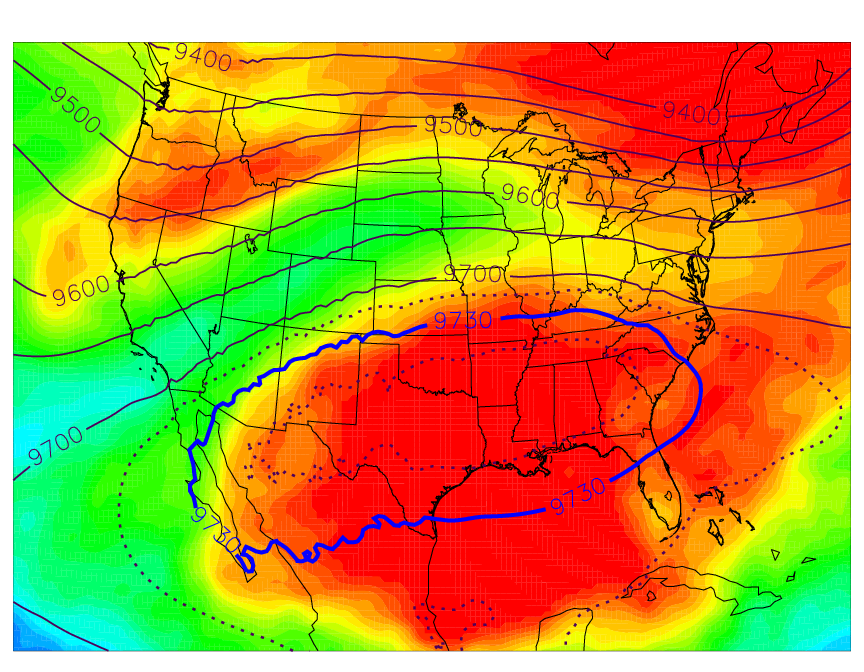
\includegraphics[width=0.48\textwidth]{o3/o308_300hPa}
		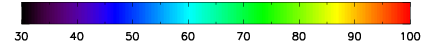
\includegraphics[width=0.48\textwidth]{o3/o3_colorbar}
		\caption[Simulated August ozone at 300\,\unit{hPa}]{{\small\textbf{Simulated upper tropospheric ozone} --- Simulated ozone
		(\unit{ppbv}) and geopotential height (\unit{m}) at 300\,\unit{hPa} averaged for August 2006. The blue 9730\,\unit{m} geopotential
		height contour indicates the ``anticylone region'' that is used throughout Chapter~\ref{ch:2006}. This figure can be compared
		to those in \citet{Cooper:2007cr}.}}
		\label{fig:2006/o3_300}
		\end{singlespacing}
	\end{wrapfigure}

Given the result from the previous section (Sec.~\ref{ssec:2006/gen/met}), we can expect to see excess tropospheric ozone provided
\chem{NO_x}-titration does not precede ozone production. Since the ozone enhancement occurs primarily above the southern
United States, it is useful to define a region of focus different from that used in Section~\ref{ssec:2006/gen/met}. Consider the
August mean geopotential height ($\bar{Z}_{300}$) at 300\,\unit{hPa} simulated by the model, we define the ``anticyclone region'' as
columns with $\bar{Z}_{300}>9730\,\unit{m}$. While the anticyclonic circulation is not stationary, using the mean circulation maximizes
the duration during which characteristics of the ozone enhancement can be captured.

Both the August mean 300\,\unit{hPa} ozone and geopotential heights are shown in Figure~\ref{fig:2006/o3_300}.
The location of ozone enhancement is consistent with that observed by \citet{Cooper:2007cr}. The ability to position the enhancement
only requires the correct dynamical features such as the anticyclone formation, which is controlled by data assimilation with NCEP
GFS inputs. North of the jet stream, stratospheric ozone appears as consistent high ozone. High ozone VMRs are observed to be mixing across
the jet stream in the outflow region (northeast corner of model domain) and circulates into the anticyclone. The finger-shaped low-ozone
structure over California separating the ozone enhancement core and northern stratospheric ozone is formed by repeated low-ozone transport from
the equatorial Pacific via the southwest corner boundary condition provided by the MOZART global CTM. Nonetheless, compared to the other studies,
the magnitude of the simulated ozone enhancement is higher by about 20\,\unit{ppbv} and slightly more widespread especially over the
Gulf of Mexico. This can be attributed to the order of magnitude over-prediction of lightning flash rate and thus {\lnox}
(see Sect.~\ref{ssec:2006/gen/met}).

	\begin{sidewaysfigure}[htbp]
		\begin{center}% yellowstone:/glade/scratch/johnwong/Dissertation
		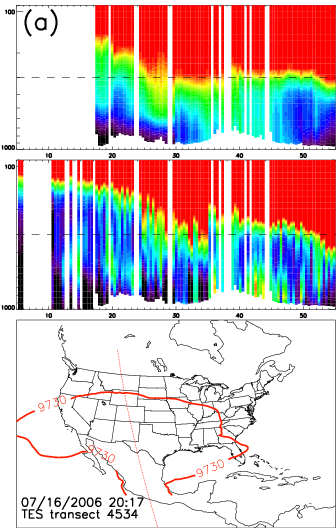
\includegraphics[width=1.6in]{o3/o3_4534_ftuv}
		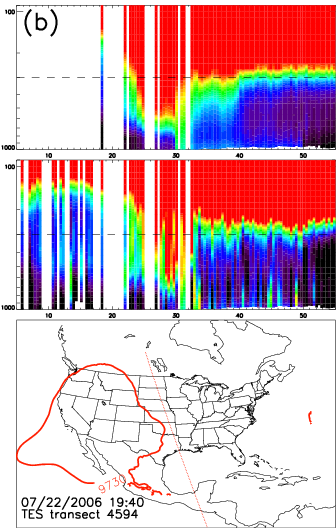
\includegraphics[width=1.6in]{o3/o3_4594_ftuv}
		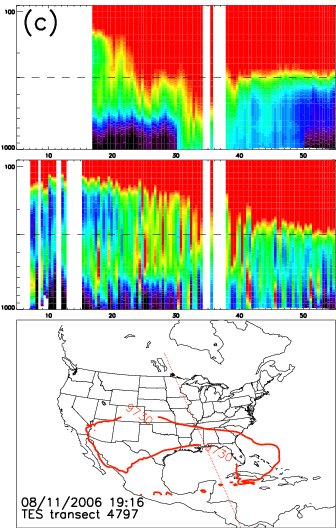
\includegraphics[width=1.6in]{o3/o3_4797_ftuv}
		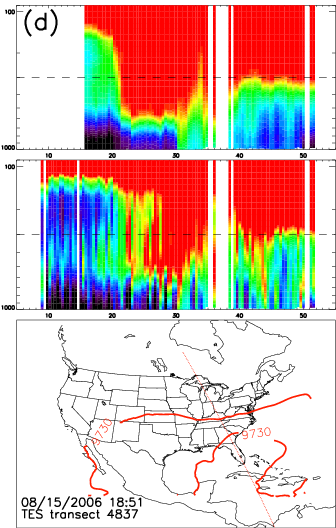
\includegraphics[width=1.6in]{o3/o3_4837_ftuv}
		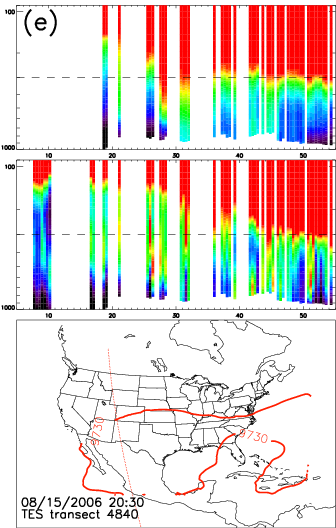
\includegraphics[width=1.6in]{o3/o3_4840_ftuv}
		
		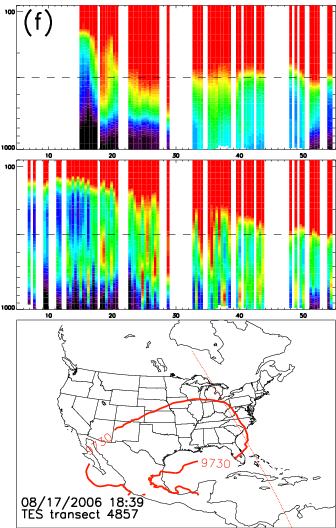
\includegraphics[width=1.6in]{o3/o3_4857_ftuv}
		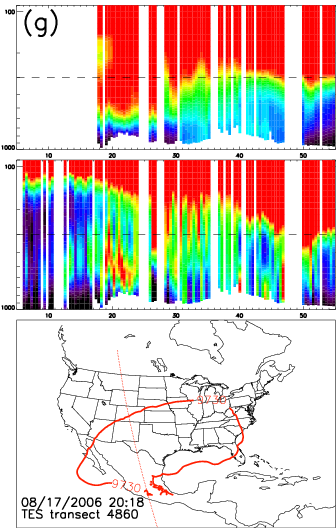
\includegraphics[width=1.6in]{o3/o3_4860_ftuv}
		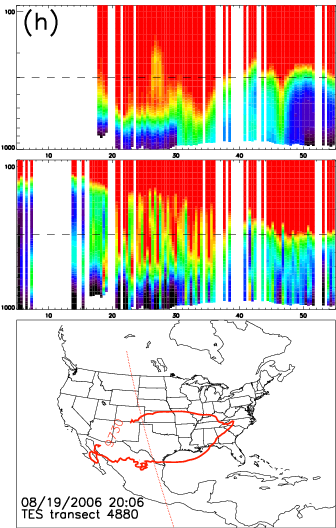
\includegraphics[width=1.6in]{o3/o3_4880_ftuv}
		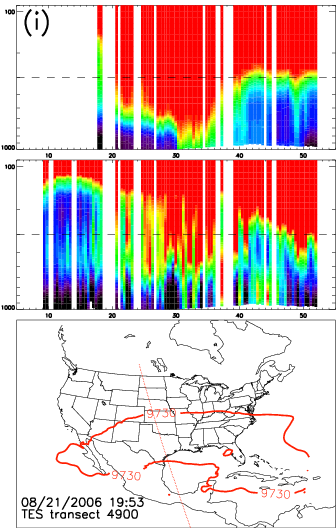
\includegraphics[width=1.6in]{o3/o3_4900_ftuv}
		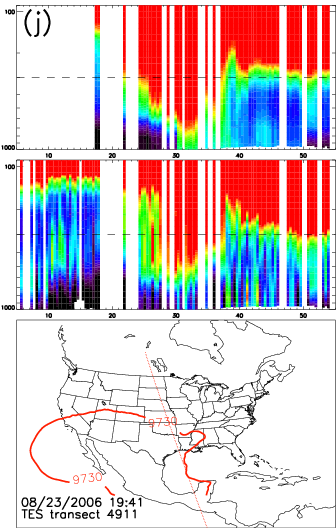
\includegraphics[width=1.6in]{o3/o3_4911_ftuv}
		
		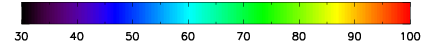
\includegraphics[width=4in]{o3/o3_colorbar}
		\end{center}
	    	\caption[TES/WRF-Chem Ozone comparisons]{\textbf{TES/WRF Ozone comparisons} --- First row for each panel is the WRF-Chem
		ozone profiles in ppbv mapped onto TES pressure coordinates after applying Equation \ref{eqn:TES-AK}. Second row is the
		TES profile. Horizontal dashed line indicates the 300\,\unit{hPa} level. Third row shows the TES transect and the  9730\,\unit{m}
		geopotential contour at 300\,\unit{hPa} from WRF. Time indicated is the 30$^\circ$N-crossing time in \unit{UTC}.} \label{fig:2006/o3tes}
	\end{sidewaysfigure}

\subsubsection{Validation against TES}

	% yellowstone:/glade/scratch/johnwong/Dissertation
	\figuremacroN{o3/o3_teswrfhist_ftuv}{WRF-Chem and TES ozone frequency distributions}{\label{fig:2006/o3tesdistr}
	Normalized frequency distributions (\unit{\%/ppmv}) of TES and WRF-Chem ozone mixing ratios between {\bf (a)}
	150--300~\unit{hPa} and {\bf (b)} 300--450~\unit{hPa}. Only columns between 25--40$^\circ$N are used.}

To quantify the bias in the simulated ozone, retrievals from the satellite-borne Tropospheric Emission Spectrometer (TES) are used
to provide spatial snapshots along selected transects. TES is a high resolution infrared Fourier-transform spectrometer with a spectral
resolution of 0.06\,\unit{cm^{-1}} \citep{Beer:2006fk}. The data products used are of V004, all of which are special observations in
step-and-stare mode with footprints of 5.3\,\unit{km}$\times$8.3\,\unit{km} and 35\,\unit{km} gaps between stares. Through comparisons
with ozonesondes, a validation with V002 showed that TES ozone had a 3--10\,\unit{ppbv} high bias in the troposphere, but it is still
able to pick up the general variability \citep{Nassar:2008mw}. TES products have been used in numerous studies on tropospheric
chemistry \citep[e.g.][]{Hegarty:2010vn,Voulgarakis:2011fk}, studies on convection and water budget \citep[e.g.][]{Brown:2008zr,Risi:2010ys},
and air quality studies \citep[e.g.][]{Mcmillan:2010kx, Wang:2011uq}.

Using TES, we first compare the ozone curtain profiles. Between July 15 and August 23, 10 TES transects are selected and compared to
the WRF-Chem output of the corresponding date at 18\,UTC or 21\,UTC, whichever is closer to the 30$^\circ$N-crossing time (Fig.~\ref{fig:2006/o3tes}).
These transects are selected because they either (a) show signals of upper tropospheric ozone enhancement, or (b) intersect regions
with 300\,\unit{hPa} geopotential height greater than 9730\,\unit{m} while passing over the United States. Of the ten transects, only transect 4594
does not satisfy criteria (b), but the TES retrieval does show a prominent upper tropospheric ozone enhancement just south of 30$^\circ$N. In
addition, to compare model outputs against TES profiles, proper transformation of the model profile is required. Let $\mathbf{x}_{\mathrm{WRF}}$
be the $\log$ of ozone column vector extracted from WRF-Chem and interpolated onto TES pressure levels, then the averaging kernel is applied
as follow:
	\begin{equation}\label{eqn:TES-AK}
		\mathbf{x}_{\mathrm{WRF}}^{\mathrm{TES}} = \mathbf{x_a} + \mathbf{A}\left(\mathbf{x}_{\mathrm{WRF}}-\mathbf{x_a}\right)
	\end{equation}
where $\mathbf{x_a}$ is the {\it a priori} constraint, $\mathbf{A}$ is the averaging kernel, and $\mathbf{x}_{\mathrm{WRF}}^{\mathrm{TES}}$
is how TES would observe the WRF-Chem ozone column. Furthermore, columns with potential problems are filtered out using the master quality
assurance flag, the C-curve flag\footnote{The C-curve flag filters out retrievals with anomalously high surface ozone \citep{Zhang:2010fk}}, and
the criteria\footnote{$trace(\mathbf{A})$ is sometimes known as the degrees of freedom for signal.}that $trace(\mathbf{A})>4.0$.
	
Figure~\ref{fig:2006/o3tes} shows the WRF-TES comparison along TES transects. Qualitatively, the height of the 100\,\unit{ppbv} ozone
isopleth is well simulated north of 30$^\circ$N. South of 30$^\circ$N, upper tropospheric ozone is often over-predicted. These over-predictions
occur either within Mexico, where the terrain of the  Sierra Madre triggers frequent large-scale thunderstorms, or the Gulf of Mexico, where {\lnox}
marine emission is unconstrained. As an example, transect 4911 (Fig.~\ref{fig:2006/o3tes}{\bf j}) is able to capture the ozone enhancement
between 28--47$^\circ$N, followed by a ridge-like low-ozone structure at 40$^\circ$N attributable to low ozone air masses transported
from the equatorial Pacific. South of 28$^\circ$N, where the transect was passing over the Gulf of Mexico, WRF-Chem is biased high
with the 100\,\unit{ppbv} ozone isopleth reaching 500\,\unit{hPa} while TES observed only 70--90\,\unit{ppbv} up to 150\,\unit{hPa}.
Similar high biases are also seen for transects 4837 (Aug 15, Fig.~\ref{fig:2006/o3tes}{\bf d}) and 4900 (Aug 21,
Fig.~\ref{fig:2006/o3tes}{\bf i}).

Comparing the upper tropospheric and mid-tropospheric ozone distribution, Figure~\ref{fig:2006/o3tesdistr} clearly shows that WRF-Chem
simulates higher ozone than observed by TES. Between 150--300\,\unit{hPa} and 25--40$^\circ$N, WRF simulated
a mean ozone mixing ratio of 123.7\,\unit{ppbv} with a standard deviation of 25.8\,\unit{ppbv} after applying the TES averaging kernel. In contrast,
TES observed $98.0\pm17.2\,\unit{ppbv}$. Therefore, WRF-Chem simulated a 21\% higher concentration of ozone within the ozone
enhancement than observed. The larger standard deviation from WRF-Chem also means that the simulated distribution has a higher
heterogeneity or less well-mixed. In the mid-troposphere, the WRF-Chem simulated and TES observed statistics are $102.1\pm26.5\,\unit{ppbv}$
and $84.8\pm18.3\,\unit{ppbv}$ respectively.

	\begin{table}[htb]
	\caption[IONS-06 August data usde]{Locations and sample sizes of IONS-06 ozonesonde August data used in this study. $N_{launches}$ is
	the number of days during August with launches performed. $N_{levels}$ is the number of vertical levels/measurements recorded during each
	launch.}
	\begin{center}
	\begin{tabular}{ccccc}\tophline
		{\bf Location} & {\bf Coordinates} & {\bf $N_{launches}$} & {\bf $N_{levels}$} & Comments \\ \middlehline
		Beltsville, MD & 39.0N, 76.5W & 7 & 3017--5196 & ${}^a$ \\
		Boulder, CO & 40.0N, 105.2W & 30 & 2451--6142 & ${}^b$ \\
		Bratts Lake, Sask. & 50.2N, 104.7W & 29 & 619--1108 & \\
		Egbert, Ont & 44.2N, 79.8W & 15 & 598--870 & \\
		Holtville, CA & 32.8N, 115.4W & 13 & 2857--6394 & ${}^b$\\
		Houston, TX & 29.7N, 95.3W & 17 & 1350--4273 & ${}^a$,${}^b$ \\
		Huntsville, AL & 34.7N, 86.6W & 29 & 4716--6622 & \\
		Kelowna, B.C. & 49.9N, 119.4W & 27 & 208--787 & \\
		Narragansett, RI & 41.5N, 71.4W & 28 & 3358--6187 & \\
		Paradox, NY & 43.9N, 73.6W & 5 & 1979--3980 & \\
		R/V R.H. Brown &  --- & 23 & 5158--9802 & ${}^a$,${}^b$,${}^c$ \\
		Socorro, NM & 34.6N, 106.9W & 25 & 2944--6684 & \\
		Table Mountain, CA & 34.4N, 117.7W & 31 & 138--4726 & ${}^b$ \\
		Trinidad Head, CA & 40.8N, 124.2W & 30 & 3752--6257 & ${}^b$ \\
		Valparaiso, IN & 41.5N, 87.0W & 5 & 2103--4129 & ${}^b$ \\
		Wallops Is, VA & 37.9N, 75.7W & 11 & 406--703 & \\
		Walsingham, Ont & 42.6N, 80.6W & 12 & 365--1108 & ${}^a$ \\
		Yarmouth, N.S. & 43.9N, 66.1W & 13 & 504--734 & \\ \bottomhline 
	\end{tabular} \label{table:2006/ions-06}
	\end{center}{
	\footnotesize
	   ${}^a$ Launched twice on certain days, only first launches (L1's) are used.
	\\ ${}^b$ Since model terminates on August 31 at 00\,\unit{UTC}, launches on August 31 are omitted.
	\\ ${}^c$ Launches from the Ronald H. Brown research vessel (R/V) on the Gulf of Mexico.
	}
	\end{table}

\subsubsection{Validation against IONS-06}

The above validation against TES shows that while ozone is overestimated, the existence of the ozone enhancement and its location is well-simulated.
Some drawbacks for using TES are the results' dependencies on {\it a priori} and their sparse temporal resolution. To complement the validation against TES,
we use ozonesonde profiles taken during the INTEX-B Ozonesonde Network Study of 2006 \citep[IONS-06;][]{Thompson:2008rp}. During this campaign,
410 ozonesondes were launched from 14 sites strategically positioned to represent major sources, sinks, and pathways of tropospheric ozone in North
America. These sondes used electrochemical concentration cell (ECC) sensors that have precision within $\pm$(5--10)\% in the troposphere
\citep{Smit:2007ta}. Between different models of the instruments, measurement biases due to variation in potassium iodide (KI) sensing concentration may be of the
order of 2--3\% \citep{Smit:2007ta}. Data from this campaign and its predecessor, IONS-04, have been used to support studies on continental tropospheric
ozone distribution \citep{Cooper:2007cr}, inferring local ozone sources \citep{Thompson:2008rp}, and comparisons with air quality model output
\citep{Tarasick:2007dq} and satellite retrievals \citep{Nassar:2008mw}.

	\begin{wrapfigure}{o}{0.5\textwidth}
		\centering
		\begin{singlespacing}
		\vspace{-.35in}
		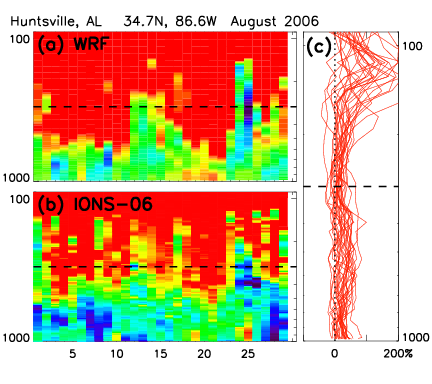
\includegraphics[width=0.48\textwidth]{o3/ions_huntsville}
		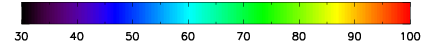
\includegraphics[width=0.48\textwidth]{o3/o3_colorbar}
		\caption[IONS-06 Huntsville launches]{\small\textbf{IONS-06 Huntsville launches} --- WRF-Chem ozone verticle profiles during August IONS-06
		ozonesonde launches at Huntsville, Alabama and the relative bias against the measured ozone mixing ratios. Horizontal dashed lines indicates
		the 300\,\unit{hPa} levels in each panel.\vspace{-.2in}}
		\label{fig:2006/ions-hunts}
		\end{singlespacing}
	\end{wrapfigure}

Ozonesondes launched during August within the model domain (Table~\ref{table:2006/ions-06}) are compared against WRF-Chem ozone columns on
WRF-Chem model grid. As an example, comparison at Huntsville, Alabama is shown in \mbox{Figure~\ref{fig:2006/ions-hunts}}. Despite the prevalent over-prediction
of ozone concentration throughout the entire troposphere, the timing of the occurrences of upper tropospheric ozone enhancement episodes correlate well
with ozonesonde measurements. Specifically, ``termination'' of the first enhancement on August 11 followed by a drop in ozone throughout the entire column
is seen in both WRF-Chem output and the ozonesonde profile. Similarly, the ``termination'' of the second enhancement on August 23/24 is also simulated. These
events are likely caused by the synoptic movement of the enhancement, controlled by dynamical features. Except for Kelowna, British Columbia, the simulated
ozone VMR above 200\,\unit{hPa} is a factor of 2--3 or higher at all North American ozonesonde sites within the model domain (not shown).

In conclusion, WRF-Chem is able to simulate an upper tropospheric ozone enhancement that coincides with the ``anticyclone region'' defined earlier, but the
overall ozone VMR is overestimated throughout the tropospheric column. Despite the high bias, spatiotemporal variabilities controlled by
large-scale dynamics are observed at individual locations affected by the ozone enhancement. Except for the three North America West Coast locations,
surface model levels, and above 200\,\unit{hPa}, tropospheric high bias rarely exceeds 100\% ($\times2$).

\subsection{Carbon monoxide}\label{ssec:2006/gen/co}

	\begin{wrapfigure}{o}{0.5\textwidth}
		\centering
		\begin{singlespacing}
		\vspace{-.15in}
		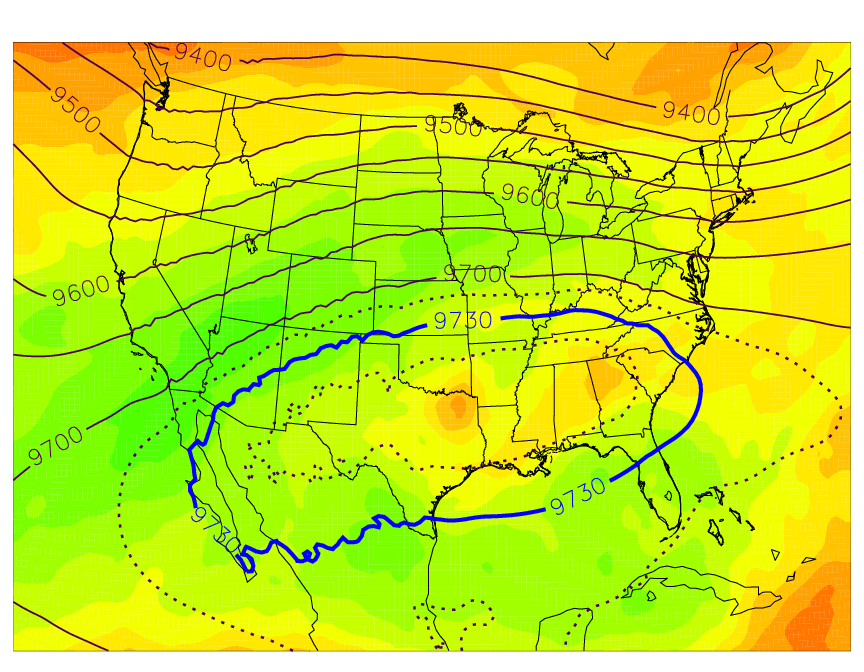
\includegraphics[width=0.48\textwidth]{co/co08_300hPa}
		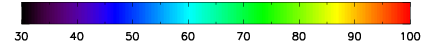
\includegraphics[width=0.48\textwidth]{o3/o3_colorbar}
		\caption[Simulated August \chem{CO} at 300\,\unit{hPa}]{{\small\textbf{Simulated upper tropospheric \chem{CO}} --- Carbon monoxide
		(\unit{ppbv}) and geopotential height (\unit{m}) at 300\,\unit{hPa} during August 2006.}}
		\label{fig:2006/co_300}
		\end{singlespacing}
	\end{wrapfigure}
	
To understand the ozone bias, it is useful to look at its chemical precursors. Carbon monoxide (\chem{CO}) is widely used for
tracking boundary layer air and pollution \citep[e.g.][]{Pan:2007sw,Weinstock:2007yj,Mcmillan:2010kx}. Emitted through incomplete
combustion, \chem{CO} is an excellent indicator for anthropogenic emission sources and biomass burning. It is also produced chemically through \chem{OH} oxidation
of a wide range of VOCs. Furthermore, its 2--3 month lifetime in the troposphere allows \chem{CO} to be an effective long-range tracer without being well-mixed.

Figure \ref{fig:2006/co_300} shows the August average \chem{CO} mixing ratio at 300\,\unit{hPa}. At the center of the NAM circulation is a distinct \chem{CO}
maximum over northeastern Texas. This feature is a combination of tracer retainment via NAM circulation and local convective detrainment of boundary layer
air. Considering the comparison performed for precipitation in Section~\ref{ssec:2006/gen/met}, this feature may be weaker if not absent due to the high bias in
convective activity in that region. On the other hand, the high \chem{CO} simulated over Georgia and neighboring states may have been underestimated because
of the under-prediction in convective activity along the Blue Ridge Mountains. North of the jet stream, anomalously high \chem{CO} is observed near the
tropopause transported from the western boundary condition defined by MOZART. This influx of \chem{CO} in the upper air can be linked to intercontinental transport
of widespread wild fires across the Siberian plateau during July.
Consistent with the transport pattern of northern high ozone, which is occasionally seen splitting off across the jet stream and transporting southwards along the
Atlantic coast and eventually merged into the ``anticyclone,'' high \chem{CO} from north of the jet stream is also observed to follow the same transport pattern.
Finally, air mass with low \chem{CO} and low ozone are transported intermittently into the domain via the southwestern boundary and into the inner CONUS
between the 9600\,\unit{m} and 9700\,\unit{m} isohypses.

\subsubsection{Validation against TES}

To evaluate the validity of the model's \chem{CO} output, we compare WRF-Chem results against TES \chem{CO} products. The instrument characteristics of TES are
already described in Section~\ref{ssec:2006/gen/ozone}. The TES \chem{CO} product has been validated against MOPITT\footnote{Measurements of Pollution in
the Troposphere.} satellite retrievals \citep{Luo:2007ly,Ho:2009lh} and aircraft measurements \citep{Luo:2007vn,Lopez:2008ys}. To summarize, TES \chem{CO}
products show slightly lower column \chem{CO} values compared to MOPITT and a $\pm10\%$ bias relative to in-situ measurements with
the primary contribution being smoothing errors and dependency on the a priori. Except for instances of poor spatiotemporal coincidences, correlation
coefficients between in-situ measurements and TES retrievals are between 0.61 and 0.92. Therefore, while retrieval values may be biased, the relative variabilities
of  \chem{CO} are expected to be realistic.

	% yellowstone:/glade/scratch/johnwong/Dissertation
	\figuremacroN{co/co_teswrfhist_ftuv}{WRF-Chem and TES \chem{CO} frequency distributions}{\label{fig:2006/cotesdistr}
	Same as Figure~\ref{fig:2006/o3tesdistr} except for carbon monoxide.}

The TES \chem{CO} product is often utilized in tandem with the TES \chem{O_3} product. \citet{Logan:2008uq} used these two products to investigate the impact
of El Ni\~no on tropospheric composition. Similarly, \citet{Voulgarakis:2011fk} used them to investigate the global \chem{O_3}-\chem{CO} correlation. Attempts
have also been made using the two TES products to characterize urban pollution outflow but was criticized for low sensitivity near the boundary layer as indicated
through its averaging kernel \citep{Shim:2007kx}. In the following validation exercise, we compare only WRF-Chem's output to the TES \chem{CO}
product using the procedure outlined in Equation~\ref{eqn:TES-AK} to mirror the comparison done with ozone in Section~\ref{ssec:2006/gen/ozone}.  Further
analysis pertaining to \chem{O_3}-\chem{CO} correlations will be revisited in Section~\ref{sec:2006/discussion}.
	
Figure~\ref{fig:2006/cotes} shows the transect-by-transect comparison of WRF-Chem \chem{CO} mapped onto TES transects against TES \chem{CO}
products. WRF-Chem is obviously biased high in the mid-to-upper troposphere. There are two possible causes for a high bias in \chem{CO}. The first being an
underestimation of the loss rate, governed by dry deposition and chemical losses via $\chem{CO}+\chem{OH}$, which may be subsequently attributed to photolysis as
$\chem{OH}$ is primarily controlled by the photolysis rate $J(\chem{O_3})$. The second possible cause is an overestimation of boundary layer air detrainment. Even though precipitation has been
under-predicted (Sect.~\ref{ssec:2006/gen/met}), there is substantial over-prediction in the frequencies of light precipitations events of $<15\,\unit{mm/day}$ (Fig.~\ref{fig:2006/precipts}).

While there is a high bias in the upper troposphere connected to convective transport, there is a low bias at northern latitudes at lower-to-mid levels
A source for these low biases is the lack of biomass burning emission via wildfire events and thus the related plume-rise vertical transport. Using the fire products from
the Moderate Resolution Imaging Spectroradiometer \citep[MODIS;][]{Justice:2002zr}, several enhanced \chem{CO} plumes in the TES transects can be identified as fire
related. On July 16, transect 4534 (Fig.~\ref{fig:2006/cotes}{\bf a}) captured a wildfire at Soda Creek, WY (43.5$^\circ$N, 110.2$^\circ$W). On August 15 and 17, multiple
transects (Fig.~\ref{fig:2006/cotes}{\bf e--g}) captured the downwind plumes of widespread fires from Oregon as heightened \chem{CO} signature between 46--53$^\circ$N.
Finally, transect 4911 captured the plume from the Idaho fires on August 23 (Fig.~\ref{fig:2006/cotes}{\bf j}). Therefore, excluding the influence of wildfire emission,
WRF-Chem is almost always biased high.

	\begin{sidewaysfigure}[htbp]
		\begin{center}% yellowstone:/glade/scratch/johnwong/Dissertation
		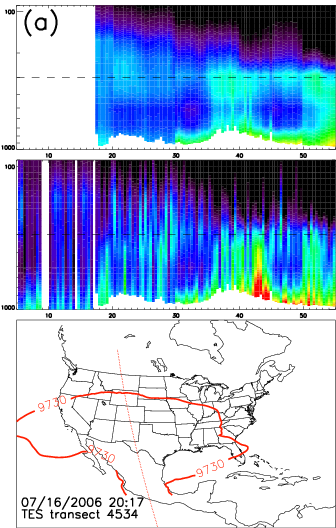
\includegraphics[width=1.6in]{co/co_4534_ftuv}
		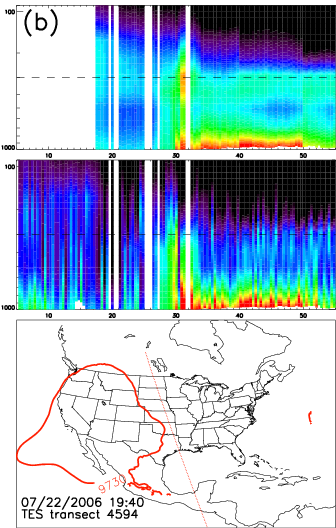
\includegraphics[width=1.6in]{co/co_4594_ftuv}
		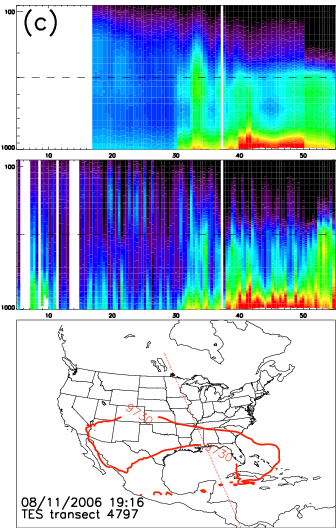
\includegraphics[width=1.6in]{co/co_4797_ftuv}
		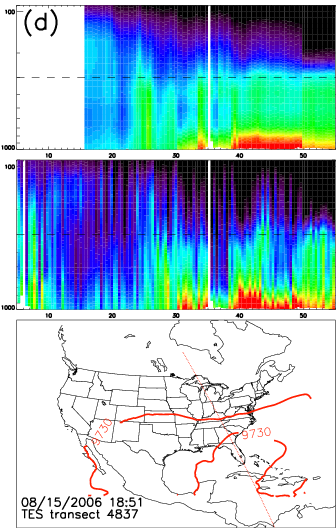
\includegraphics[width=1.6in]{co/co_4837_ftuv}
		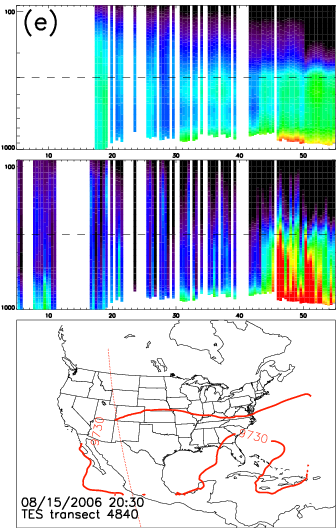
\includegraphics[width=1.6in]{co/co_4840_ftuv}
		
		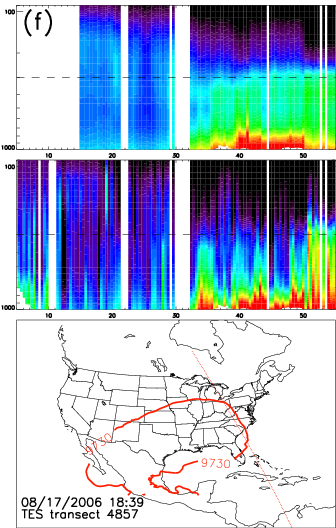
\includegraphics[width=1.6in]{co/co_4857_ftuv}
		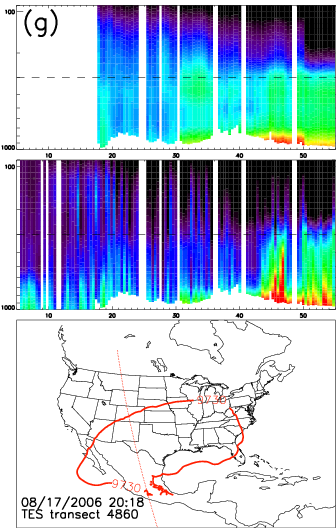
\includegraphics[width=1.6in]{co/co_4860_ftuv}
		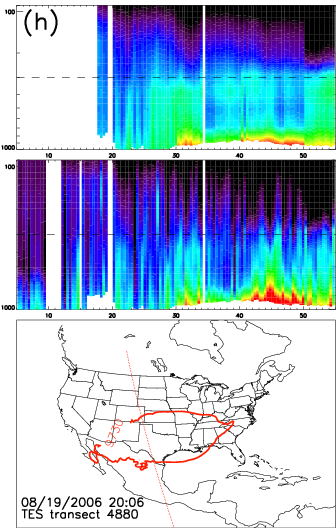
\includegraphics[width=1.6in]{co/co_4880_ftuv}
		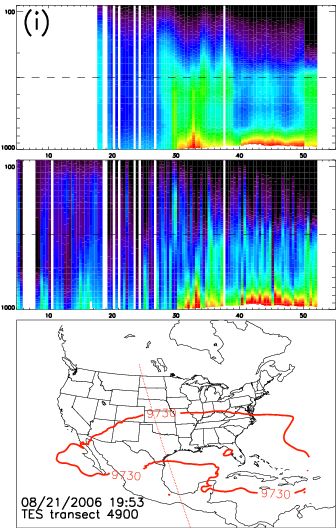
\includegraphics[width=1.6in]{co/co_4900_ftuv}
		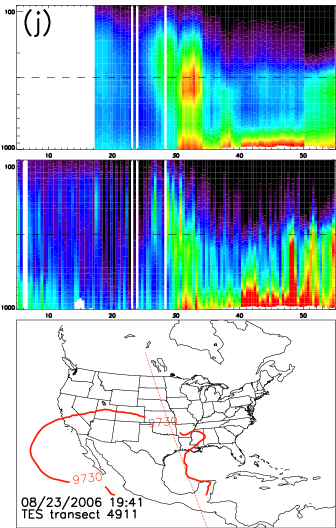
\includegraphics[width=1.6in]{co/co_4911_ftuv}
		
		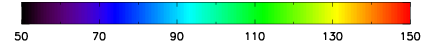
\includegraphics[width=4in]{co/co_colorbar}
		\end{center}
	    	\caption[TES/WRF-Chem \chem{CO} comparisons]{\textbf{TES/WRF \chem{CO} comparisons} --- Same as Figure~\ref{fig:2006/o3tes} except for carbon
		monoxide.} \label{fig:2006/cotes}
	\end{sidewaysfigure}

Considering only data between 25--40$^\circ$N, the frequency distributions between WRF-Chem and TES retrievals are shown in Figure~\ref{fig:2006/cotesdistr}. The
computed mean values for the upper tropospheric distributions are 81.7\,\unit{ppbv} and 67.7\,\unit{ppbv} for WRF-Chem and TES respectively, and thus WRF-Chem is
20.7\% too high. In addition, the standard deviations of the distributions are significantly different with 11.7\,\unit{ppbv} for WRF-Chem and 14.3\,\unit{ppbv} for TES. In other words,
WRF-Chem is more well-mixed than TES. In the mid-troposphere, the mean VMRs are 94.6\,\unit{ppbv} and 81.3\,\unit{ppbv}, thus WRF-Chem is 16.3\% higher. Similar
to the upper troposphere, the standard deviations also show that WRF-Chem is more well-mixed. It is worth noting that the disparity in \chem{CO} spatial heterogeneity between
WRF-Chem and TES is surprisingly consistent with the validation done by \citet{Barth:2012qf} despite the differences in mean VMR bias and targeted pressure level.

There are at least three possible causes for these biases. The first being wildfire plumes, which intermittently introduce outliers in the TES distribution but not in WRF-Chem's.
Another cause, which is debatable, may be that of a longer residence time for \chem{CO} in WRF-Chem than the actual value. Given
the excessive $J(\chem{O_3})$ (Apdx.~\ref{a-sec:bug/ftuv}), it may be hypothesized that \chem{OH} is underestimated and excess {\lnox} is responsible for consuming too much
\chem{HO_x} to form various reservoir nitrogen species such as \chem{HNO_3} and \chem{HONO}. The model biases in \chem{NO_x} will be discussed in Section~\ref{ssec:2006/gen/nox}. Finally,
a TES transect has a 7.5\,\unit{mrad} or 5.3\,\unit{km} cross-track Field of View (FoV), which is to be compared with the 36\,\unit{km} grid spacing in WRF-Chem. Therefore, TES
observations are highly susceptible local variabilities and outliers.

%WRF_UT:      81.6672      138.012      1.40809      3.88935
%TES_UT:      67.6742      205.599     0.593247      1.44802
%WRF_MT:      94.5807      129.222      1.57465      4.29820
%TES_MT:      81.3291      187.742     0.365582     0.886847

\subsubsection{Validation against MOPITT}

Measurements of Pollution in the Troposphere (MOPITT) is a satellite-borne instrument with the primary mission of measuring tropospheric \chem{CO}. MOPITT is a
multi-channel gas correlation radiometer \citep{Drummond:1996ve}. It uses a maximum a posteriori (MAP) algorithm for retrieval \citep{Deeter:2003bh}. It has a
horizontal resolution of 22 km $\times$ 22 km and 7 pressure levels. Improvements to the forward model such as consideration of variability in modulation cell pressure
are incorporated in version 4 \citep{Deeter:2010dq}. This study uses version 5, which has been validated by \citet{Deeter:2013fk}. After accounting for the different
retrieval methods, and consequently different a priori and averaging kernels, MOPITT produces roughly the same CO volume mixing ratio and column density as TES
within $\pm15\%$ \citep{Luo:2007ly}. Though having lower spatial resolution, MOPITT offers slightly higher sensitivity than TES close to the boundary layer and a larger
FoV, which complements the \chem{CO} products from TES with valuable cross-track information.

\figuremacroW{co/mopitt_compare}{WRF and MOPITT \chem{CO} comparisons}{
\label{fig:2006/mopitt}Comparison of WRF-Chem \chem{CO} $\log_{10}$VMR ($y$) against MOPITT $\log_{10}$ retrievals ($x$) for the indicated dates and pressure
levels. Pre-logarithm units are \unit{ppbv}. Red asterisks are the centers of mass calculated using the geometric means of the two parameters. Diagonal blue lines indicate
the identity line. Only data between 12--18\,\unit{UTC} are used.}{.9}

Figure~\ref{fig:2006/mopitt} shows the WRF-Chem \chem{CO} outputs ($y$), after applying the MOPITT equivalent of Equation~\ref{eqn:TES-AK}, plotted against MOPITT
retrievals ($x$) at 4 different pressure levels and 3 dates. To minimize diurnal biases, only morning (12--18\,\unit{UTC}) data are used. The total number
of columns that lie within the model domain during the given timeframe are 3168, 3693, and 4983 for the 3 days. It is clear that WRF-Chem is performing very poorly in the upper troposphere relative
to MOPITT. There is practically no correlation above 700\,\unit{hPa}. The distributions are, nonetheless, consistent with prior validations against TES, wherein WRF-Chem
\chem{CO} has been found to be more well-mixed (vertically) than observed. With this comparison, WRF-Chem is shown to have too much mixing horizontally as well.
Considering the means, contrary to previous validations against TES, WRF-Chem is shown to slightly under-estimate \chem{CO} at 300\,\unit{hPa}, albeit
only by $-4.4\%$, $-1.7\%$, and $-3.2\%$ for the three days validated. At lower levels, the positive bias in WRF-Chem increases, but so are the correlations with MOPITT. On the
surface, the mean biases are $+17.7\%$, $+19.6\%$, and $+27.8\%$.

In conclusion, WRF-Chem \chem{CO} is almost uniformly biased high compared to satellite retrievals except in the presence of wild fire emission plumes. Comparisons against
TES and MOPITT show that \chem{CO} is predicted to be more well-mixed horizontally and vertically than observations. Constrained by anthropogenic emission sources and coastal boundaries,
PBL \chem{CO} VMRs enjoy high correlations between model and remote sensing data. However, this correlation rapidly drops off for higher altitudes

\subsection{Formaldehyde}\label{ssec:2006/gen/form}

Unlike \chem{CO}, formaldehyde (\chem{HCHO}, or \chem{CH_2O}) has a much shorter residence time of $O$(hours) in the atmosphere. Besides chemical production
from methane, the primary source for \chem{HCHO} is isoprene, which
is emitted by plants, thus \chem{HCHO} has been used as a proxy for constraining spatial distributions of biogenic emissions. \citep[e.g.][]{Palmer:2006qf,Millet:2008oq,Marais:2012kl}.
In addition, \chem{HCHO} may also be emitted through industrial combustion and construction processes. Additional description of anthropogenic and biogenic VOCs are given
in Section~\ref{ssec:intro/ozone/voc}.

	% yellowstone:/glade/scratch/johnwong/Dissertation
	\begin{wrapfigure}{o}{0.5\textwidth}
		\centering
		\vspace{-.3in}
		\begin{singlespacing}
		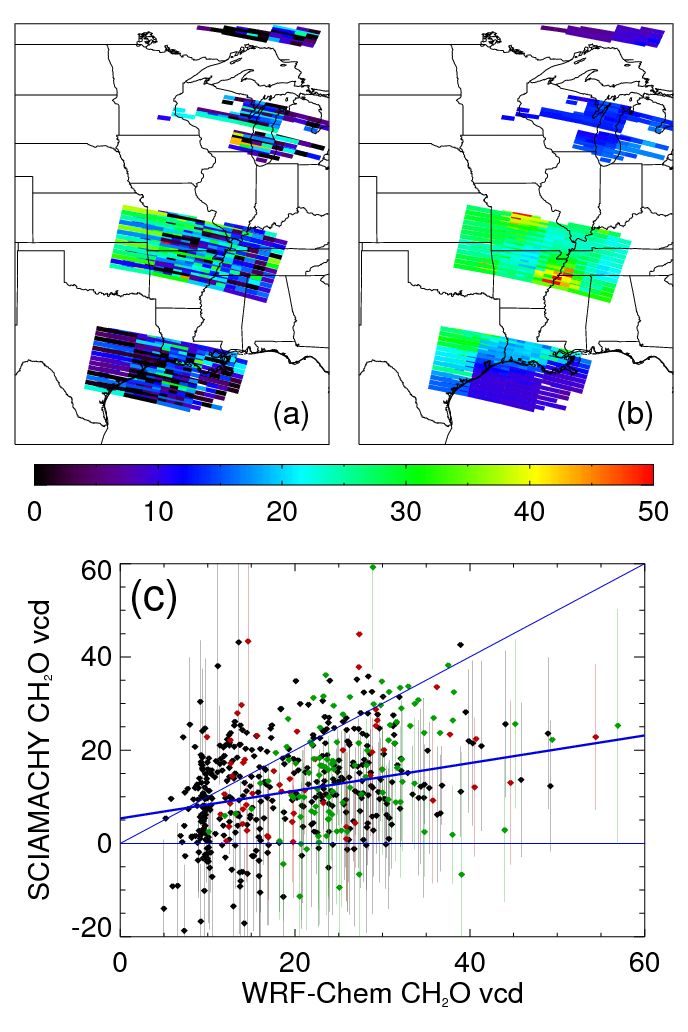
\includegraphics[width=0.48\textwidth]{scia_ch2o_compare_0818}
		\caption[SCIAMACHY and WRF-Chem formaldehyde on 8/18]{{\small\textbf{SCIAMACHY and WRF-Chem formaldehyde on 8/18} --- \textbf{(a)} SCIAMACHY and
		\textbf{(b)} WRF-Chem \chem{HCHO} tropospheric VCDs in $10^{15}\,$\unit{molecules\,cm^{-2}} for August 18. \textbf{(c)} Both VCDs plotted against each other.
		Red data points represent anthropogenic sources on the surface. Green data points represent biogenic sources. Blue lines are $y=x$, best-fit, and $y=0$.}}
		\label{fig:2006/scia_hcho_0818}
		\end{singlespacing}
		\vspace{-.2in}
	\end{wrapfigure}

Formaldehyde can be monitored from space using the Scanning Imaging Absorption Spectrometer for Atmospheric Chartography (SCIAMACHY) instrument, an imaging
spectrometer on board of the Environmental Satellite (ENVISAT) with an emphasis of monitoring regions with intense biomass burning or anthropogenic pollution
\citep{Burrows:1995fk,Bovensmann:1999uq}. It measures scattered and reflected sunlight in the thermal IR spectral range, providing sensitivity to trace gases in the
troposphere such as \chem{HCHO} and \chem{NO_2}. The retrieval for the data used in this study is developed at the Royal Netherlands Meteorological Institute (KNMI)
and provided by the Tropospheric Emission Monitoring Internet Service (TEMIS) project (\url{http://www.temis.nl}). Using near-UV radiance measurements and global
CTM outputs to provide a priori, \chem{HCHO} tropospheric vertical column densities (VCDs) are retrieved and constrained using a Differential Optical Absorption
Spectroscopy (DOAS) technique \citep{De-Smedt:2008uq}. SCIAMACHY \chem{HCHO} products have also been used for determining long time trends \citep{De-Smedt:2010kx} as
well as assimilated to constrain model isoprene \citep{Dufour:2009fk}.

Using the Ozone Monitoring Instrument \citep[OMI;][]{Levelt:2006kl}, \citet{Millet:2008oq} found that most of the high \chem{HCHO} VCDs are located at approximately east of
96$^\circ$W and south of 40$^\circ$N for July--August 2006. Therefore, we focus on SCIAMACHY scans overpassing this region. In particular, we use two overpasses
on August 18 (track ID 23355) and August 24 (23441) at approximately 16\,\unit{UTC} as examples due to timing and location coincidence of features of interest
to this study. The averaging kernels show a mean peak sensitivity between 200--300\,\unit{hPa} with moderate sensitivity close to the surface ($\sim50\%$ at 700\,\unit{hPa}).
To calculate the simulated retrieval error in the VCD, the following equation is used \citep[after][]{Boersma:2004uq,De-Smedt:2008uq}:
\begin{equation}\label{eqn:hcho_vcde}
	\sigma^2_{N_v} = \frac1{M^2}\frac{\sigma^2_{N_s,r}}{n}+\frac{1}{M^2}\sigma^2_{N_s,s}+\left(\frac{\Delta N_s}{M^2}\right)^2\sigma^2_M+\sigma^2_{CTM}
\end{equation}
where $\sigma_{N_s,r}$ and $\sigma_{N_s,s}$ are the random and systematic slant column errors, $M$ is the air mass factor, $N_v$ and $N_s$ are the VCD and slant column
density (SCD), $n$ is the number of satellite pixels used, and $\sigma_{CTM}$ is the error in the reference background from using a CTM during retrieval.

Figure \ref{fig:2006/scia_hcho_0818} shows the pixel-by-pixel comparison of the SCIAMACHY \chem{HCHO} tropospheric VCDs and the WRF-Chem \chem{HCHO} VCDs
weighting using the SCIAMACHY averaging kernels. All model data points captured by each pixel's bounding polygon are selected and the SCIAMACHY
averaging kernel is applied to the geometric mean. In an attempt to classify whether biases are originated from biogenic or anthropogenic sources, data
points are highlighted as green if the corresponding model grid-box has a MEGAN isoprene emission factor $>75\,\unit{mol/km^2/h}$, i.e. substantial biogenic emission. Those
highlighted as red correspond to columns with surface anthropogenic \chem{HCHO} emission at the 95-percentile from the weekday EPA NEI-08 (see
Sect.~\ref{ssec:intro/ozone/voc} and Sect.~\ref{ssec:2006/method/chem} for more details). Due to MEGAN's vegetation mapping, biogenic and anthropogenic sources are not
mutually exclusive. In cases where both criteria are satisfied, the data point is colored green because of the higher molar emission rate. It should be noted that such categorization of data points
is not absolute. Due to transport, non-anthropogenic grids can also see heavy anthropogenic influences. On the other hand, due to the high altitude of SCIAMACHY's maximal
sensitivity, pixels expecting high sources of surface emission may not display high VCD when the model is not simulating sufficient lofting.

Similar to the results from the \chem{CO} validation in Section~\ref{ssec:2006/gen/co}, WRF-Chem also over-predicts \chem{HCHO}. However, due to $\sigma_{N_v}$ being large
for most data points, 71\% (391/550) of the pixels\footnote{Error bars for these data points are removed from Fig.~\ref{fig:2006/scia_hcho_0818} to avoid overcrowding the figure.}
shown in Figure~\ref{fig:2006/scia_hcho_0818} satisfied $|N_{v,WRF}-N_{v,SCIA}|<\sigma_{N_v}$. The minimized-$\chi^2$ fit to the data set gives a slope of 0.297, which loosely
implies WRF-Chem predicting three times more \chem{HCHO} in the atmosphere than observed by SCIAMACHY. Despite the over-estimation, this snapshot sample shows
a background value of $10^{16}$\,\unit{molecules\,cm^{-2}} and a mean of $2.06\times10^{16}$\,\unit{molecules\,cm^{-2}}, which are consistent with OMI and GEOS-Chem
\citep{Millet:2008oq}.

	% yellowstone:/glade/scratch/johnwong/Dissertation
	\begin{wrapfigure}{o}{0.5\textwidth}
		\centering
		\vspace{-.4in}
		\begin{singlespacing}
		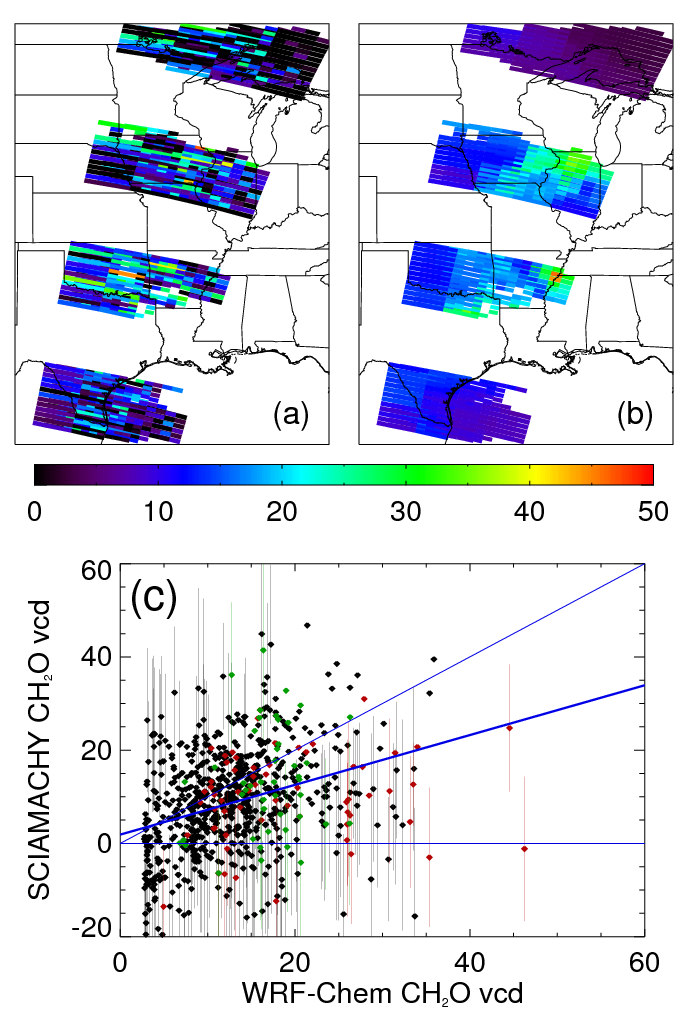
\includegraphics[width=0.48\textwidth]{scia_ch2o_compare_0824}
		\caption[SCIAMACHY and WRF-Chem formaldehyde on 8/24]{{\small\textbf{SCIAMACHY and WRF-Chem formaldehyde on 8/24} --- Same as
		Figure~\ref{fig:2006/scia_hcho_0824} except for August 24.}}
		\label{fig:2006/scia_hcho_0824}
		\end{singlespacing}
		\vspace{-.3in}
	\end{wrapfigure}

More specific features can also be extracted. For instance, a \chem{HCHO} local VCD high corresponding to Memphis, Tennessee can be found in the model output but not in the
SCIAMACHY retrieval. On the contrary, two single-pixel maxima in the SCIAMACHY retrievals associated with Little Rock, Arkansas and Springfield, Missouri cannot be identified
in the model output. This is primarily due to lowering the resolution of EPA NEI-08 data as an input for emission, which subsequently dilutes relatively small urban sources while
leaving metropolitan-sized sources intact. However, considering the relative impact of the larger biogenic sources versus small urban sources of formaldehyde, such bias is not expected
to have any noticeable influence in the long-term simulated chemistry.

On August 24 (Fig.~\ref{fig:2006/scia_hcho_0824}), two stationary fronts lingered between the two southern footprints and between the two northern footprints. They generated
some convective systems, which caused the missing pixels, but otherwise did not affect the remaining views. Of the 767 pixels available on this day, 612 (79.8\%) are within $\pm1\sigma_{N_v}$
of the identity line. The minimized-$\chi^2$ fit gives a slope of 0.53, which loosely means that WRF-Chem is over-predicting by a factor of 2, compared to the factor of 3 on August 18.
Among the large patch of low VCD pixels to the north, the background value is roughly $3\times10^{15}$\,\unit{molecules\,cm^{-2}}. This is low compared to the \citet{Millet:2008oq}
seasonal average, but still reasonable compared to SCIAMACHY's retrieval. Otherwise, the rest of the data points are well within the seasonal averages in this area. Similar to August 18,
Memphis can again be identified as a spatially isolated formaldehyde source that appears as an outlier in the WRF-Chem distribution but not the SCIAMACHY distribution.

\subsection{Nitrogen Oxides}\label{ssec:2006/gen/nox}

Considering that CG flash rate is over-predicted by a factor of 10 (see Sect.~\ref{ssec:2006/gen/met}), it is expected
that \chem{NO_x} is also substantially over-predicted for the southeastern United States. Indeed, when examining
within the anticyclone region,  the \chem{NO_x} VMR is increased by an order of magnitude  within the first few days
of the simulation (Fig.~\ref{fig:2006/nox}). While the initial condition from MOZART provides an average of 300\,\unit{pptv}
of \chem{NO_x} at 300\,\unit{hPa} within the anticyclone, it is increased to 2\,\unit{ppbv} by July 5. Consistent with the hypothesized attribution to tropospheric
{\lnox} emission, the increase in \chem{NO_x} is only observed within the troposphere below $\sim100\,\unit{hPa}$
but peaks near 200\,\unit{hPa} where the maximum convective detrainment level typically occurs for larger systems.

To evaluate the model's output, we compare tropospheric \chem{NO_2} VCDs against SCIAMACHY's retrieval from
KNMI TEMIS. Similar to the formaldehyde retrieval, the algorithm employs the Differential Optical Absorption Spectroscopy
(DOAS) method and a data-assimilation technique, which utilizes a chemistry-transport model (CTM) with ECMWF
operational analyses meteorology to estimate the stratospheric portion of the retrieved column \citep{Boersma:2004uq}.
Validation of the TEMIS \chem{NO_2} product has been performed by \citet{Lambert:2004aa} against NDSC data, showing
bias up to $3.5\times10^{15}$ molec cm$^{-2}$. The differences between retrievals have been attributed mostly to the
tropospheric air mass factor (AMF$_{trop}$) used \citep{vanderA:2010aa}, which has a sensitivity to cloud fractions of
up to 20\% \citep{Boersma:2004uq}.

\figuremacroN{noxcol}{WRF-Chem \chem{NO_x} VMR}{\label{fig:2006/nox}{\bf (a)} Average \chem{NO_x} VMR within
the anticyclone region during July 2006 showing sharp increase towards a higher steady state within the first few days
of the simulation. {\bf (b)} VMR time-series at 300\,\unit{hPa} showing a sample of the temporal variability within the anticyclone.}

Considering the transient nature of storms and the model's skill in predicting the exact locations and magnitudes of individual
convective cores over the entire 2-month simulation at a relatively low resolution, this comparison will be performed over a large
number of orbits as opposed to individual retrieval as done in the previous section for formaldehyde (Sect.~\ref{ssec:2006/gen/form}).
However, since the pixel size is relatively small and almost always contained within a model grid, each pixel is only associated
with a single model column determined by directly mapping to the WRF Lambert conformal grid. Corresponding
WRF-Chem output is determined by rounding the time of measurement to the nearest 3-hour. Due to ENVISAT's orbit, all
measurements are taken between 15--21\,\unit{UTC}. Matched WRF-Chem \chem{NO_2} partial columns
are then accumulated using the tropospheric VCD averaging kernel defined as $A_{trop} = A\cdot AMF/AMF_{trop}$, where
$A$ is the total column VCD averaging kernel, for levels below the provided tropopause index computed using the WMO
tropopause definition. These VCDs, together with the associated retrieval biases and SCIAMACHY VCDs,  are then
accumulated back onto the WRF model grid. Over 61 days, $5.2\times10^5$ pixels were selected, accounting for $\sim1\%$
of all pixels globally over the same period. Individual model grid receives anywhere between 0 to 15 pixels, which is less
than 20 ($\approx$61 days/3 days per global survey) due to rejected measurements.

	\begin{table}
		\begin{center}
		\begin{singlespacing}
		\caption[Linear regression on $NO_2$ VCDs]{Using $VCD=4.39\times10^{15}$\,\unit{molec.\,cm^{-2}} as a
		threshold, the following statistics summarize the two partitons.}
		\begin{tabular}{cccccc} \tophline
		Partition&  $n(\%)$ & Regression & $r^2$ & $\chi_{reduced}^2$ & $P(>\chi_{reduced}^2)^\dagger$ \\
		\middlehline
		$VCD>4.39$ & 29997 (58.1\%) & $y=2.76+2.21x$ & $0.09$ & $51.76$ & $\sim0$ \\
		$VCD<4.39$ & 21641 (41.9\%)  & $y=0.49+0.42x$ & $0.332$ & $0.911$ & $\sim1$ \\
		\bottomhline
		\end{tabular}
		\label{tab:2006/no2reg}
		\end{singlespacing}
		\end{center}
		{\footnotesize ${}^\dagger$ Probability that a fit has a reduced-$\chi^2$ higher than the given fit. High $P$'s correspond to ``good'' fits.}
	\end{table}

Using this procedure, the frequency distributions of WRF-Chem and SCIAMACHY KNMI \chem{NO_2} tropospheric VCDs
are calculated (Fig.~\ref{fig:2006/no2vcd}{\bf a}). While the WRF-Chem distribution is lognormal with a background close
to $0.1\times10^{15}$\,\unit{molec.\,cm^{-2}}, the SCIAMACHY distribution is closer to a normal distribution skewing towards
the left with a negative tail. Negative values in tropospheric column is permitted because of the retrieval process, which
involves estimating and subtracting the \chem{NO_2} stratospheric column. Despite the differences in the distributions, the modes
for both distributions are close to $0.5\times10^{15}$\,\unit{molec.\,cm^{-2}}, consisting mostly of data points from the Pacific
marine columns, Idaho/Montana, and Canada. These regions have low contributions from \chem{NO_x} of anthropogenic or 
lightning sources, thus making them less susceptible to biases in emission inventory and lightning parameterization. On the
contrary, but as expected, the WRF-Chem substantially over-estimates the $>2\times10^{15}$\,\unit{molec.\,cm^{-2}}
range, which corresponds to levels typically observed only at locations with persistent anthropogenic sources. Because of the
high bias in lightning emission, \chem{NO_2} VCDs over the southeastern United States and Mexico are severely over-estimated
(Fig.~\ref{fig:2006/no2vcd}{\bf c\&d}).

Using the passive decaying {\lnox} tracer, described in Section~\ref{ssec:2006/method/diagnostics}, each tropospheric VCD
data point can be classified as below or above half of the median {\lnox} tracer tropospheric VCD ($\approx4.39\times10^{15}$
\unit{molec.\,cm^{-2}}) computed using the SCIAMACHY averaging kernel (Fig.~\ref{fig:2006/no2vcd}{\bf b}). The results from
attempting to perform linear regressions on the data points are summarized in Table~\ref{tab:2006/no2reg}. The upper partition
($VCD>4.39$), which corresponds to a high level of {\lnox} tracer in the model, correlates poorly with SCIAMACHY retrievals with
a reduced-$\chi^2=52$. The mean ratio of WRF-Chem VCD to SCIAMACHY VCD is 4.9, i.e. $\chem{NO_2}$ level is 5 times higher
than observed when the region is heavily influenced by {\lnox} emission. On the contrary, the lower partition ($VCD<4.39$) shows
good correlation between the model and observation with $\chi_{reduced}^2=0.911$. For this category, WRF-Chem over-predicted
\chem{NO_2} by only \chem{17\%} when lightning is minimally involved.

Finally, the above model-observation comparison should be interpreted with caution as there are numerous factors that prevent literal
interpretations. One factor is the frequency distribution of VCDs. While the model shows a lognormal-like distribution,
SCIAMACHY's retrieval introduces a negative tail. Since negative values in tropospheric VCD is meaningful and represents a crucial
property of the retrieval process, they cannot be filtered out and must be included in the overall statistics. However, the exact
interpretation of these non-physical negative VCDs remain ambiguous.

\figuremacroW{scia_no2}{WRF-Chem and SCIAMACHY \chem{NO_2} VCDs}{\label{fig:2006/no2vcd}
{\bf(a)} Frequency distributions of WRF-Chem and SCIAMACHY \chem{NO_2} tropospheric VCDs in $10^{15}$\,\unit{molecules\,cm^{-2}} during July and August 2006.
{\bf(b)} A log-log plot of the two tropospheric VCDs partitioned into halves by median passive lightning tracer tropospheric VCDs and their corresponding linear minimized-$\chi^2$ fits and correlation
coefficient $r^2$.
{\bf(c)} Spatial distribution of mean WRF-Chem tropospheric VCDs in $10^{15}$\,\unit{molecules\,cm^{-2}}. With pixel density indicating the number of samples used to compute
the mean (up to $n=15$ but saturates at $n=10$) at each model grid point.
{\bf(d)} Same as {\bf c}, but for SCIAMACHY.}{0.9}

\vspace{1.2in}

\noindent The ozone level is sensitive to the balance between VOC and \chem{NO_x} (Sect.~\ref{ssec:intro/ozone/nox}). In
Section~\ref{ssec:intro/ozone/nox}, it is shown that (CG) lightning is over-predicted by a factor of 10 under the assumption of a constant
CG fraction of $1/4$. Together with the validation results from the previous sections (Sect.~\ref{ssec:2006/gen/co} \& \ref{ssec:2006/gen/form}),
the model is expected to simulate an both excess VOCs and excess \chem{NO_x} relative to observation, thereby explaining the
over-estimation of ozone shown in Section~\ref{ssec:2006/gen/ozone}. By comparing model \chem{CO} (Sect.~\ref{ssec:2006/gen/co}),
formaldehyde (Sect.~\ref{ssec:2006/gen/form}), and \chem{NO_2} (Sect.~\ref{ssec:2006/gen/nox}) against remote sensing profiles, it is
indeed shown that both VOCs and \chem{NO_x} are definitively over-estimated, though due to intricacy of the validation methods, the
numerical results from the comparisons may not be construed with absolute certainty. Nonetheless,  by accounting for these biases, the
analyses done in Section~\ref{sec:2006/discussion} will proceed with caution and will frequently reference individual result from this
section when appropriate.

\section{Discussion}\label{sec:2006/discussion}

\section{Sensitivity study}\label{sec:2006/sens}
\subsection{Anthropogenic emission}\label{ssec:2006/sens/anthrop}
\subsection{Biogenic emission}\label{ssec:2006/sens/bio}
\subsection{Lightning emission}\label{ssec:2006/sens/lnox}

\section{Conclusions}\label{sec:2006/conslusion}